\documentclass[11pt]{article}

\marginparwidth 0.5in
\oddsidemargin 0.25in
\evensidemargin 0.25in
\marginparsep 0.25in
\topmargin 0.25in
\textwidth 6in
\textheight 8in

\usepackage{amsmath, amssymb}
\usepackage{upgreek}
\usepackage{latexsym}
\usepackage{graphicx}

\begin{document}
\begin{flushleft}
Juan Miguel C. Manalo \\
2014-40093 \\
CS 145 THWMXY-HONOR
\end{flushleft}

\begin{center}
\textbf{CS145 Lab Exercise 1: Wireshark Lab - Getting Started} 
\end{center}

\section*{Part 1}
\begin{quote}
\begin{enumerate}
\item{Some of the protocols listed are \textbf{HTTP}, \textbf{TCP}, and \textbf{SSL}.}
\item
HTTP GET \textit{(\#175)}: $75.815245s$ or $15:50:10.682221$ \\
HTTP OK \textit{(\#176)}: $75.819832s$ or $15:50:10.688808$ \\
TIME: $0.004587s$
\item
IP Address (Website): 10.16.5.225 \\
IP Address (Computer): 10.40.80.35
\item
The two packets referred to in the second question are marked in red (Packets 175 and 176, respectively), along with the time at capture. They are also the basis for the answers in the third question. If we consider \textbf{HTTP GET}, then the source is the computer (blue) and the destination is the website (green).
\begin{center}
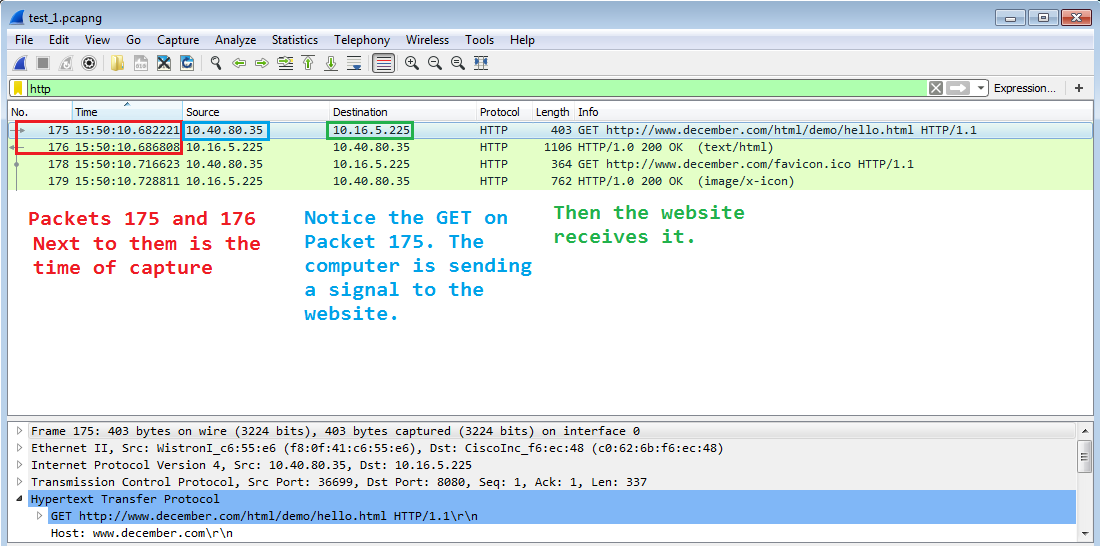
\includegraphics[scale=0.5]{LEPic_1D}
\end{center}

\end{enumerate}
\end{quote}

\section*{Part 2}
\begin{quote}
\begin{enumerate}
\item
The two websites are \textbf{www.vatican.va/} and \textbf{w2.vatican.va/content/vatican.html}, highlighted in the screenshots below (Packets 598 and 618).

\begin{center}
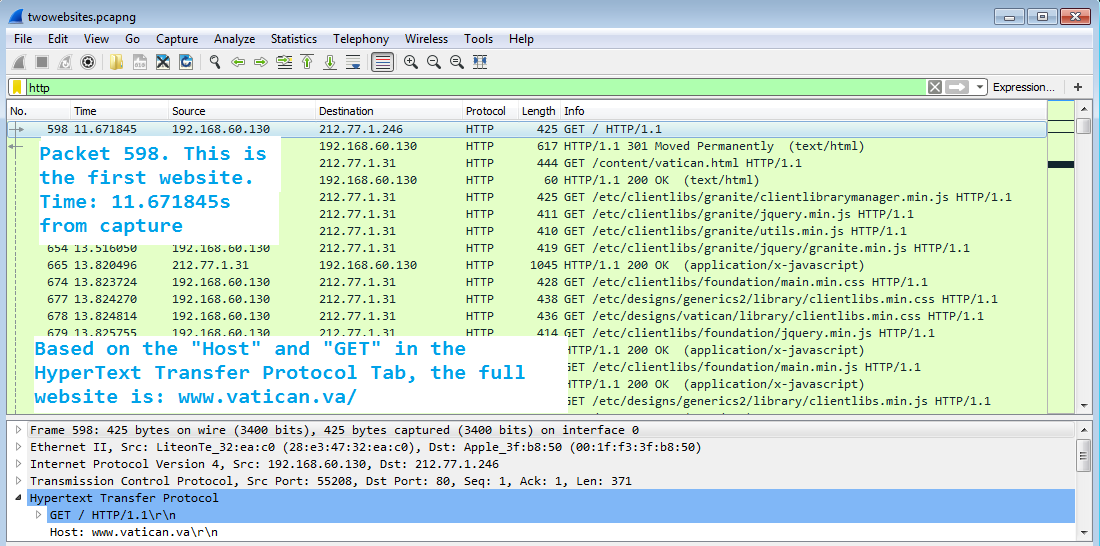
\includegraphics[scale=0.5]{LEPic_2A_1}
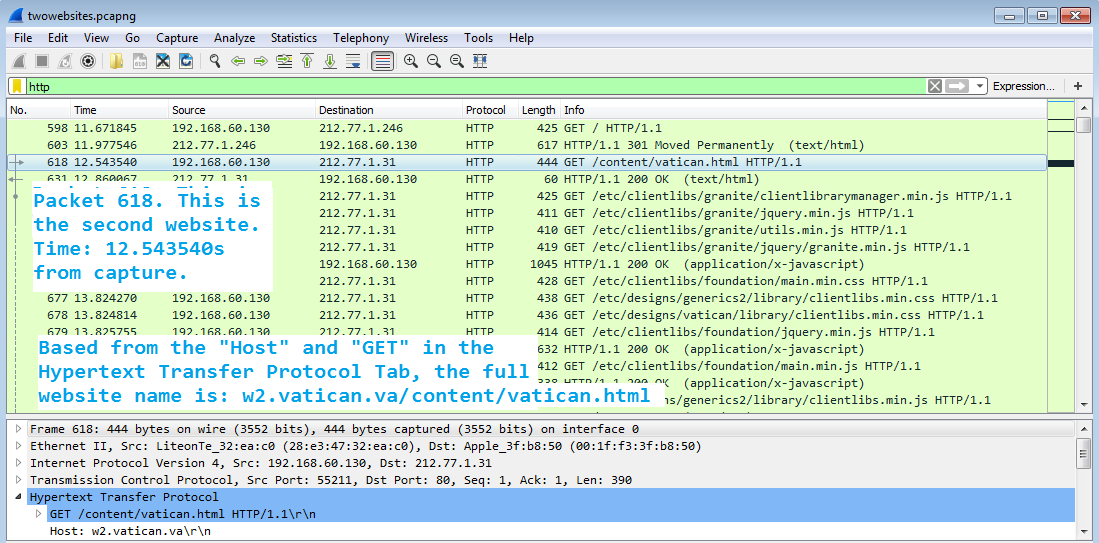
\includegraphics[scale=0.5]{LEPic_2A_2}
\end{center}

\item
IP Address (Computer): 192.168.60.130 (highlighted red in the screenshot).

\begin{center}
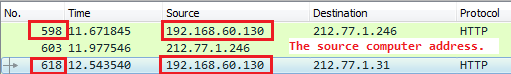
\includegraphics[scale=1]{LEPic_2B}
\end{center}
\end{enumerate}
\end{quote}

\end{document}